{
%\makeatletter % to change template
%    \setbeamertemplate{headline}[default] % not mandatory, but I though it 
%%was 
%    %better to set it blank
%    \def\beamer@entrycode{\vspace*{-\headheight}} % here is the part we are 
%    %interested in :)
%\makeatother
\setbeamertemplate{headline}
{\vspace*{-\headheight}
}
\usebackgroundtemplate{
%\setlength{\unitlength}{1em}
%\begin{picture}(1em,2em)
%\put(10em,10em){ 
\includegraphics[width=4em]{npsglobe}
%}
%\end{picture}
\hspace{-1em}
\begin{picture}(250,250)
\put(0,0){
\begin{tikzpicture}
\node (img1)  at (0,0) 
{
\includegraphics[width=1.25\textwidth]{backgroundlight}};
\end{tikzpicture}
}
\put(280,0){
\begin{tikzpicture}
\node (img1)  at (0,0) 
{
\includegraphics[width=15em]{npsglobe}};
\end{tikzpicture}
}
\put(200,150){
\begin{tikzpicture}
\node (img1)  at (0,0) 
{
\includegraphics[scale=0.25]{npslogovert}};
\end{tikzpicture}
}
\put(0,0){
\begin{tikzpicture}
\node (img1)  at (0,0) 
{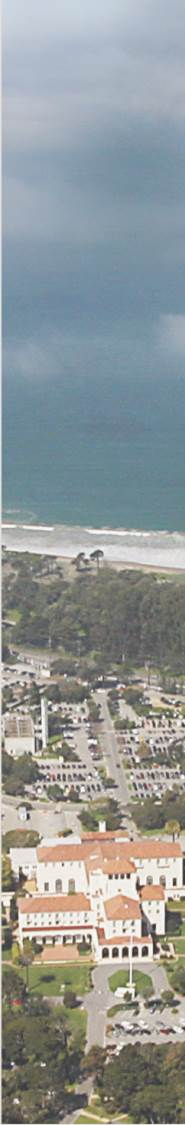
\includegraphics[height=\textheight]{sidepicture}};
\end{tikzpicture}
}
\end{picture}
}
\begin{frame}
\titlepage
\end{frame}
}